%09.10.2024, lecture 2

\section{One-way functions}\label{sec:one_way_functions}


$\fP$ means functions that can be computed in polynomial time.
$\FP$ means to find a solution in polynomial time.

\begin{definition}
    A one-way function is an injection function that can be easily computed (in polynomial time), but it cannot be inverted easily (in polynomial).
\end{definition}

\begin{theorem}
    Let $\PP \neq \NP$, then there is $f \in \fP$ such that $f^{-1} \not \in \FP$.
\end{theorem}
\begin{proof}
    Let $\Phi$. be a Boolean formula.
    Let $A \in \{0, 1\}^n$ be a Boolean assignment to its $n$ variables.
    Define
    \begin{align*}
        f(\Phi, A) = \begin{cases}
        (\Phi, 1^n), &\text{ if } \Phi[A]=1 \\
        (\Phi, 0^n), &\text{ if } \Phi[A]=0
        \end{cases}
    \end{align*}
    If we could invert $f$, we could solve SAT by computing $f^{-1}(\Phi, 1^n)$.

    So, if $\PP \neq \NP$ and $f, f^{-1} \in \fP$, hence $\PP = \NP$.
    And vice versa, if $f \in fP, f^{-1} \not\in \fP$, hence we can solve SAT and $\PP = \NP$.
    %TODO complete proof
\end{proof}

\begin{statement}
    The are $2^{2^n}$ functions $\{0, 1\}^n \to \{0, 1\}^*$ and $2^{O(n \cdot 2^{\sqrt n})}$ circuits of size $\leq 2^{\sqrt n}$.
\end{statement}

\begin{exercise}
    Almost all length-preserving functions have \"similar\" circuit complexity in both directions.
\end{exercise}

It means that one-way functions are rare.

We will define one-way functions formally.
Let $f \colon \{0, 1\}^n \to \{0, 1\}^*$.
Consider family of sliced functions: $f_i \colon \{0, 1\}^i \to \{0, 1\}^i$.
And more general $f_i \colon \{0, 1\}^{n(i)} \to \{0, 1\}^{m(i)}$ for some polynomials.
\begin{definition}
    We say that function $f \colon \{0, 1\}^* \to \{0, 1\}^*$ with slices $\{f_n\}_{n \in \N}$ is \emph{one-way} if:
    \begin{itemize}
        \item $f_n \colon \{0, 1\}^n \to \{0, 1\}^n$ can be computed in time $\poly(n)$.
        \item For every polynomial-time randomized adversary $A$, for every $k$
        \[
            \Pr[A(f_n(x)) \text{ inverts } f_n] < \frac 1 {n^k},
        \] here $\Pr$ is over $x$ from $U_n$ and $A$'s randomness.
    \end{itemize}
\end{definition}

Adversary's algorithm can be uniform or non-uniform (circuit).
This does not matter for us in most cases.
We will try to highlight when it matters.

\begin{definition}
    Sequence $t_1, t_2, \ldots$ is \emph{negligible} if for every $k$ and every $n$ large enough,
    \[
        t_n < \frac 1 {n^k}.
    \]

    And non-negligible if there is $k$ such that for every $n$ large enough, $t_n \geq \frac 1 {n^k}$
\end{definition}


On practice, one would like to be able to invert his function but at the same time wants that others cannot invert it.
Hence, we need the next definition.
\begin{definition}
    \emph{One way function family (owff)} is a deterministic polynomial-time algorithm $G \colon (1^n, r_g) \to (s_n, e_n)$ that generates two Boolean circuits:
    \begin{itemize}
        \item $e_n \colon \{0, 1\}^n \to \{0, 1\}^{m(n)}$ (the function itself)
        \item $s_n \colon \{0, 1\}^{\sigma(n)} \to \{0, 1\}^n$ (sampler, takes random bits and produces some distribution)
    \end{itemize}
    such that for all $A$ (adversary, randomized poly-time) and $\forall k \in N \; \exists N \colon \forall n > N$
    \[
        \Pr[A(e_n(s_n(r_s)), 1^n, e_n, s_n) \in e^{-1}(e_n(s_n(r_s)))] < \frac 1 {n^k},
    \] where $\Pr$ is over $A$'s randomness and uniformly distributed $r_g, r_s$.
    Basically it says that over function cannot be easily inverted.
    See \Cref{fig:2fc91310-fbf1-4d04-abdb-24f1fdf8893a}.
 \begin{figure}[H]
        \centering
        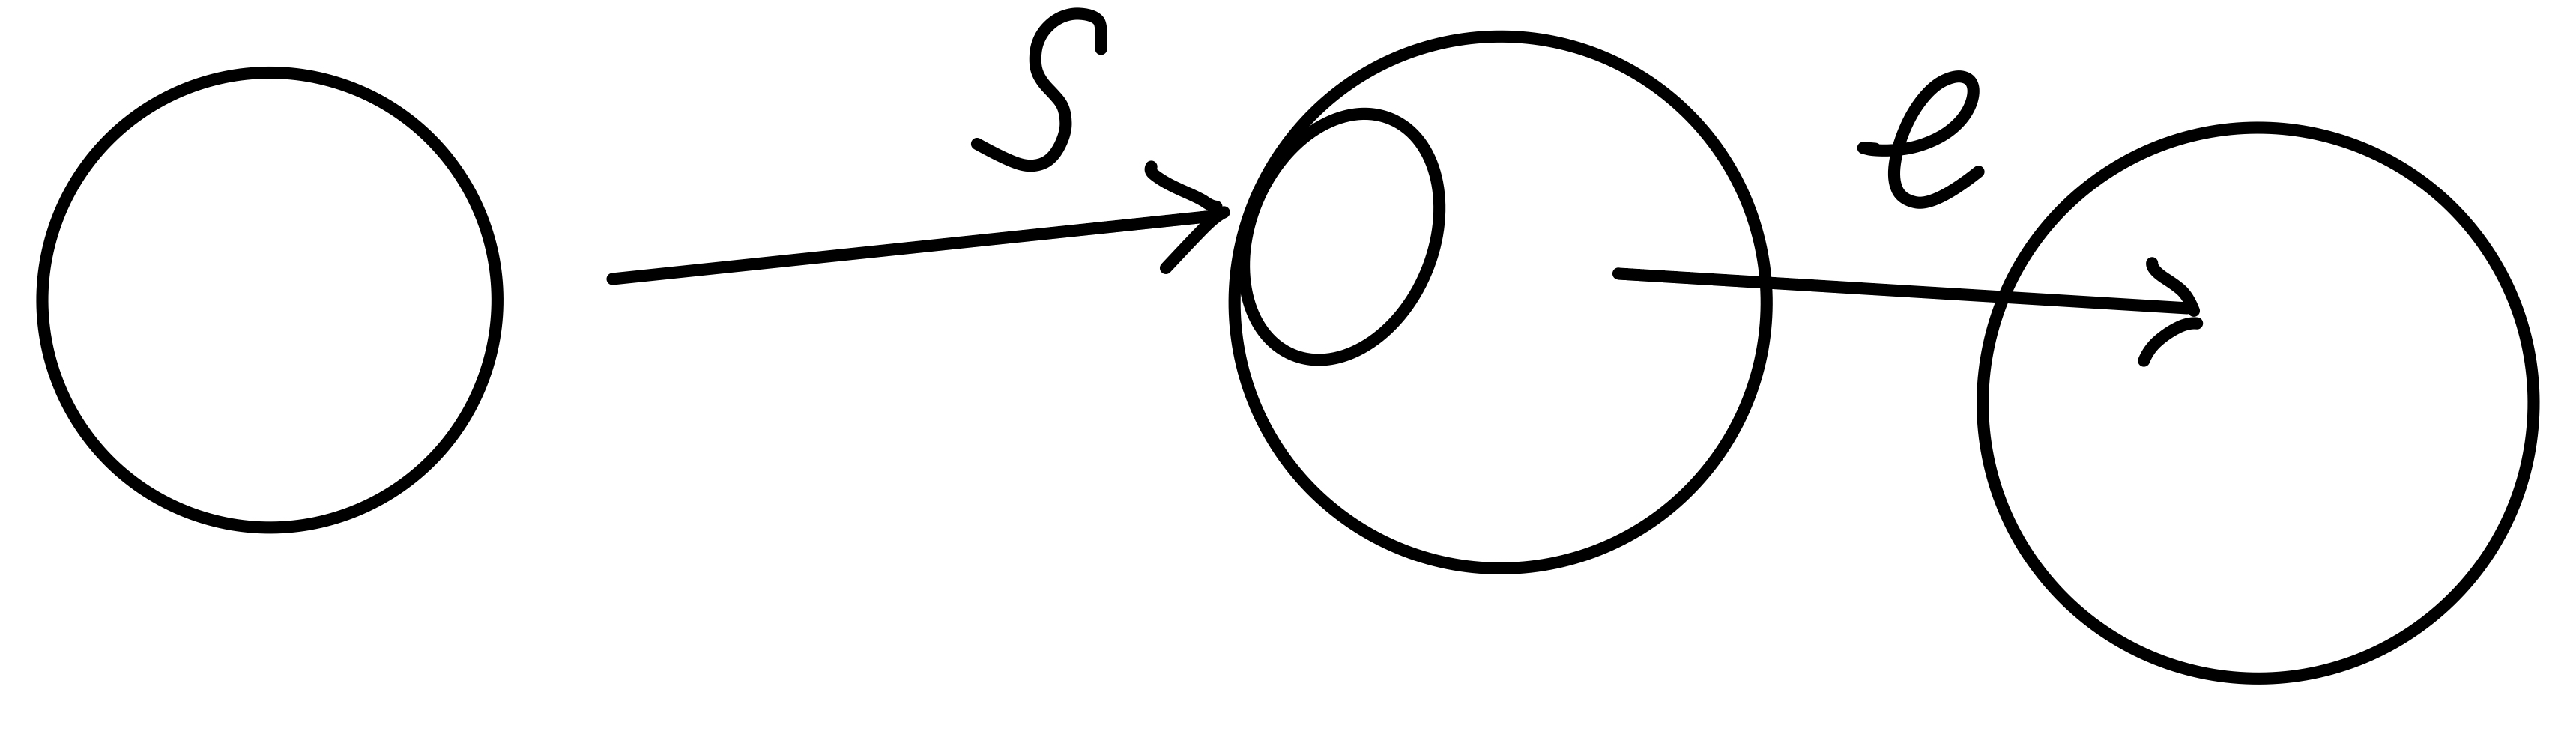
\includegraphics[width=0.4\textwidth]{figures/2FC91310-FBF1-4D04-ABDB-24F1FDF8893A}
        \caption{Schema.}
        \label{fig:2fc91310-fbf1-4d04-abdb-24f1fdf8893a}
    \end{figure}
\end{definition}

Usually our owf's will be nice:
\begin{itemize}
    \item length-regular: $|x| = |y| \implies |f(x)| = |f(y)|$ (typically),
    \item length-preserving: $|f(x)| = |x|$ (sometimes),
    \item length-poly-bounded: $|x|^{\Omega(1)} \leq |f(x)| \leq |x|^{O(1)}$ (always),
    \item not necessarily defined on each length,
    \item can be goodly sliced.
\end{itemize}

\begin{definition}
    \emph{Strong owf} is an owf such that for all $k$ an adversary cannot reach success probability $1/n^k$.

    \emph{Weak owfs} are such that $\exists k$ an adversary cannot reach success probability $1/n^k$.
\end{definition}

\begin{theorem}
    Each weak owf can be transformed into strong owf.
\end{theorem}
\begin{proof}
    Let $f_w$ be a weak owf.
    \[
        f_s(x_1, \ldots x_m) = (f_w(x_1), \ldots, f_w(x_m)),
    \]
    for some polynomial $m = m(n) = \Omega(n)$.

    Assume that $A_s$ inverts $f_s$ with $\Pr \geq 1/n^k$.
    We will construct $A_w$ that breaks $f_w$.
    $A'_w(y)$:
    \begin{itemize}
        \item for each $j \in [m]$,
        \item take $x_1, \ldots, x_m$ at random,
        \item let $x = A_s(f_w(x_1), \ldots, f_w(x_{j - 1}), y, f_w(x_{j + 1}), \ldots, f_w(x_m))_j$,
        \item if $f_w(x) = y$, return $x$.
    \end{itemize}
    Final $A_w$ repeats $A'_w(y)$ for $a(n)$ times and returns the majority answer.
    The concrete polynomial will be given later.

    Let $S$ be a success set for $A'_w$:
    \[
        S = \{y \in \{0, 1\}^n \mid \Pr[A'_w \text {inverts } f_w \text{ in } y] > \frac n {a(n)}\}.
    \]
    Hence, overall success of $A_w$ is at least
    \begin{align*}
        \Pr[y \in S] &\cdot \underbrace{\Pr[A_w \text{ inv. } f_w \text{ in } y \mid y \in S]}_{1 - (1 - \frac 1 {a(n) / n})^{a(n)}} \approx \\
        &\approx \Pr[y \in S] \cdot \left(1 - \frac 1 {e^n}\right).
    \end{align*}
    \begin{claim}
        $\Pr[x \in S] \geq 1 - \frac 1 {mn}$, where $m$ is a number of copies.
    \end{claim}
    As we prove it the probability of success would be enough to break $f_w$ as we choose $m$.
    \begin{proof}
        Assume that $\Pr[x \in S] < 1 - \frac 1 {mn}$.
        \[
            \Pr[A_s \text{ succeeds}] \leq \Pr[x_i \in S \; \forall i \in [m]] + \Pr[\text{success if not all in } S].
        \]
        \begin{itemize}
            \item Since $\Pr[x \in S] < 1 - \frac 1 {mn}$ we have \[
                      \text{All } \leq ((1 - \frac 1 {m/n})^{m/n})^n \approx \frac 1 {e^n}.
            \]
            \item \[\text{Not all } \leq \frac n {a(n)} \cdot m\].
            Because $y \not \in S$ and we try $m$ times to extract the answer.
        \end{itemize}
        Let $a(n)$ be much, much bigger than $m$.
    \end{proof}

\end{proof}

\begin{example}
    Let $f(a, b) = a \cdot b$.
    It can invert a lot of times simply because $a \cdot b$ is usually disible by two.
\end{example}

\begin{example}
    Let $f(p, q) = p \cdot q$, where $p, q \in \mathbb P$, $p < q$ and $\log p \approx \log q$.
\end{example}

\begin{example}
    \[
        f(x_1, \ldots, x_n, I) = (x1, x2, \ldots, x_n, \sum_{i \in I} x_i]),
    \] where $I \subseteq [n]$.
\end{example}

\begin{example}[Discrete logarithm]
    Take $p \in \mathbb P$.
    Take $g$ a generator in $\mathbb F_p$.
    Consider $x \in \Z_{p - 1}$.
    And let
    \[
        f(x) = g^x \mod p.
    \]
    It is called logarithm since to invert it we need to find $\log_g(g^x)$.
\end{example}

\begin{definition}
    We say that $f$ can be reduced to $g$ ($f \to g$) is there is randomized poly-time algorithm $T^{\bullet}$ such that.
    For all $k_f$ there is $k_g$ and any adversary $A$ such that.
    If $A$ inverts $g$ with $\Pr \geq 1 - \frac{1}{n^{k_g}}$, then there is some $T^A$ that inverts $f$ with $\Pr \geq 1 - \frac{1}{n^{k_f}}$.
\end{definition}

\begin{theorem}[Universal one-way function]
    There is a universal weak one-way function $u$, i.e. $\forall f \in \fP$ it implies that $f \to u$.
\end{theorem}
\begin{proof}
    Let $u(M, x) = (M, M(x))$, where $x \in \{0, 1\}^*$ and $M$ is a description of a Turing machine.
    And $M(x)$ is the output of $M$ on $x$ within $|x|^2$ steps (just to be able to compute $u$).
    \begin{lemma}
        Without loss of generality, a weak owf is computable in $|x|^2$ steps.
    \end{lemma}
    \begin{proof}
        Let $\tilde f(x_1, x_2) = f(x_1) \circ x_2$, where $|x_1| = n, |x_2| = m = m(n)$.
        We choose $m(n)$ such that $(|x_1| + |x_2|)^2$, hence we can compute $\tilde f$ in $|x|^2$ time.
    \end{proof}

    We will demonstrate that if we can invert $f^*$ computed by $M^*$ using an inverter for $u$.
    After we fixed $M^*$, the proportion of inputs of the form $(M^*, \cdot)$ is a constant (because we fixed a prefix).
    Hence, we still can invert a large proportion of inputs for $f^*$.
\end{proof}

\begin{exercise}
    What about strong owf?
\end{exercise}

\begin{exercise}
    What about when we have deterministic or non-uniform adversaries?
\end{exercise}

\subsection{Trapdoor function}

Simply we define a function that we can invert, but nobody else couldn't.
\begin{definition}
    \emph{Trapdoor function family (tdff)} is a collection of poly-time functions $e_n, d_n$ such that $d_n(e_n(x)) = x$ and for every adversary $A$,
    \[
        \Pr[A \text{ inverts } e_n \text{ in } x] \text{ is neglibible}.
    \]
\end{definition}
The problem is that there is no uniform algorithm $D(n, x)$ for $d_n$ since it is not invertible in polynomial time.
More accurate one:
\begin{definition}
    Tdff is a deterministic poly-time $G \colon (1^n, r_g) \to (e, s)$ (Boolean circuits) such that:
    \begin{itemize}
        \item $e \colon \{0, 1\}^n \to \{0, 1\}^{s(n)}$ (encryptor)
        \item $d \colon \{0, 1\}^{s(n)} \to \{0, 1\}^n$ (decryptor)
        \item $s \colon \{0, 1\}^{\sigma(n)} \to \{0, 1\}$ (sampler),
    \end{itemize}
    such that for all $x \in \Im(s)$ we have $d(e(x)) = x$ and for all adversary $A$ we have.
    For all $k \in \N$ there is $N$ such that for all $n > N$,
    \[
        \Pr[A(e(s(r_s)), 1^n, e, s) \in e^{-1}(e(s(r_s)))] < \frac 1 {n^k},
    \] where $G(1^n, r_g) = (e, d, s)$ and $\Pr$ is taken over $A$'s randomness and over uniformly distributed $r_g, r_s$.
\end{definition}
Basically, the most difficulty is in the random bits.
Having $e$ and knowing which bits were used we can invert it.
But without knowing them it is hard.

\begin{example}[RSA, Rivest-Shamir-Adleman]
    Take $p, q \in \mathbb P$ (secret).
    let $N = p \cdot q$ (known to everyone).
    Pick $\eps, \delta$ from $\Z_N$ such that $\eps \cdot \delta = 1 \mod (p - 1)(q - 1)$ (secret).
    And let $s(x) = x, \; e(x) = x^{\eps} \mod N, \; d(x) = x^{\delta} \mod N$.
\end{example}
\begin{proof}
    Let's show that it works:
    \[
        d(s(x)) = x^{\eps \delta} \mod N = x \mod N.
    \] By Fermat's theorem.
\end{proof}